\documentclass[a4paper,11pt]{article}
\usepackage[francais]{babel}
%% Prévu pour compiler avec lualatex
% \usepackage[utf8]{inputenc}
\usepackage{fontspec}
\usepackage{libertine}
% \usepackage[T1]{fontenc}
\usepackage{graphicx}
\usepackage{fancyhdr}
\usepackage[top=2.5cm, bottom=2.5cm, left=2cm, right=2cm]{geometry}
\usepackage{listings}
\usepackage[utf8]{luainputenc}
\usepackage[hidelinks]{hyperref}
\usepackage{caption}

\lfoot{\bsc{Enseirb-Matmeca}}
\rfoot{Informatique --- 3\ieme{} année}

\pagestyle{fancy}
\begin{document}

\begin{titlepage}
  \begin{center}

    \begin{center}
      
\includegraphics[width=4cm]{EM.jpg}
    \end{center}

    \vspace*{1cm}
        
    \rule{0.75\linewidth}{0.7mm}\\[0.4cm]
    {\Huge Rapport TP1 --- PVM\\[0.4cm]}
    \rule{0.75\linewidth}{0.7mm} \\[1.5cm]

    {\Large Bazire \bsc{Houssin}\\Sylvain \bsc{Vaglica}\\Stéphane \bsc{Castelli}\\[2cm]}
    {\Large Mardi 29 Octobre 2013}
  \end{center}
\end{titlepage}

\tableofcontents
\clearpage
\section{Introduction}

PVM est une bibliothèque C et Fortran permettant la communication entre des processus sur une machine parallèle ou un cluster de machines ; elle utilise pour cela un démon lancé sur chaque machine qui se charge du routage des messages, du contrôle des processus et des problèmes pouvant survenir.Créée en 1989, PVM a au fil des décennies perdu en popularité au profit de MPI, mais reste un moyen efficace d'apporter une solution à des problèmes dont la résolution en séquentiel mettrait trop de temps. Au travers de ce projet, il a été réalisé un système distribué de craquage de mot de passe en force brute, sur le modèle maître / esclaves, avec un processus maître créant et distribuant des tâches, et des processus esclaves les exécutant. Un des objectifs principaux du projet, en plus de nous initier à la communication inter-processus et plus particulièrement à PVM, est d'analyser et optimiser la création et la répartition des tâches afin d'obtenir les meilleures performances possibles. Il sera d'abord explicité les choix qui ont été effectués, puis ils seront analysés.


\section{Nombre de solutions}

Un mot de passe peut se définir par sa complexité. Celle ci peut être augmentée facilement par deux moyens : l'augmentation de la longueur maximale et l'augmentation du cardinal de l'alphabet utilisé. En effet, si l'on cherche un mot de passe sans le connaître, par force brute, il faut tester chacune des possibilités dans un ensemble donné, et plus il y a de mot de passes possibles dans cet ensemble, plus la tâche est longue à réaliser pour un ordinateur. Un mot de passe de longueur $k$ sur un alphabet de $n$ lettres fournit ainsi $n^k$ possibilités à tester. Par conséquent, si l'on connaît l'alphabet et que l'on se fixe une longueur maximale de mot de passe à tester $l$, alors on a dans le pire des cas :

\[
\sum_{k=0}^{l}n^k = \frac{n \cdot (n^l - 1)}{n - 1} = \mathcal{O}(n^l)
\]

Dans le cas qui nous concerne, l'alphabet est les lettres minuscules comprises entre \emph{a} et \emph{o}, soit 15 lettres. On a donc :

\[
\sum_{k=0}^{l}15^k = \frac{15 \cdot (15^l - 1)}{14} = \mathcal{O}(15^l)
\]

Même si cela limite la quantité de possibilités, on peut remarquer que leur nombre croît de manière exponentielle avec la longueur. En conséquence de quoi, au dela d'une certaine valeur il devient impossible pour une machine actuelle de terminer la recherche en un temps raisonnable. Toutefois, la parallèlisation du code et l'utilisation de PVM permettent de repousser cette valeur.

\section{Représentation des données}

%gmp
%type de données transmis
%conversion entier/mdp


\section{Le maître}
Il s'occupe de démarrer les processus esclaves et de leur assigner les tâches. Le processus maître commence par envoyer à chaque esclave le mot de passe en clair, puis transforme l'ensemble des mots de passe possibles en un intervalle d'entiers (fonction bijective décrite dans la partie précédente). Chaque fois qu'un esclave demande du travail, il lui assigne un sous intervalle de l'intervalle initial, en lui donnant le début de l'intervalle et un pas (nombres d'entiers à tester).
Une gestion dynamique du pas est essentielle pour équilibrer le travail des esclaves et garantir une exécution la plus rapide possible. En effet, il est essentiel que l'ensemble des esclaves terminent le plus proche possible les un des autres.

\section{Les esclaves}
Chacun reçoit quand il le demande, un intervalle d'entiers correspondant à un certain nombre de mot de passe possibles à tester.
En effet, pour chaque entier de l'intervalle, l'esclave le convertit en une chaine de caractère et le compare ensuite grâce à la fonction \texttt{strcmp()} , au mot de passe réel reçu en argument lors de la création des processus esclaves par le maître. Si le résultat est positif, l'esclave communique au maître que l'exécution doit terminer car le mot de passe a été trouvé. Sinon, il continue jusqu'à arriver à la fin de son intervalle. Il communique alors avec le processus maître pour recevoir un nouvel intervalle de travail.


\section{La répartition des tâches}
% choix des intervalles
% demande de travail des esclaves
% attribution


\section{Changements en version multi-threadée}

\section{Performances}
\begin{figure}[h!]
  \centering
  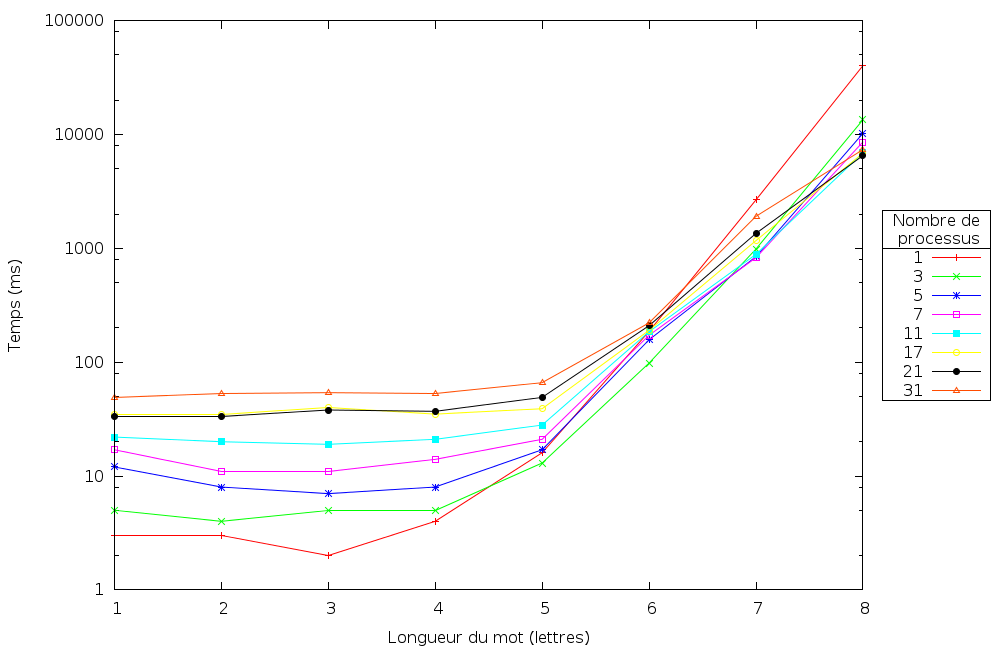
\includegraphics[width=\textwidth]{plot_log.png}
  \caption{Tests de performance, représentés sur une échelle logarithmique}
  \label{perf_loga}
\end{figure}

\begin{figure}[h!]
  \centering
  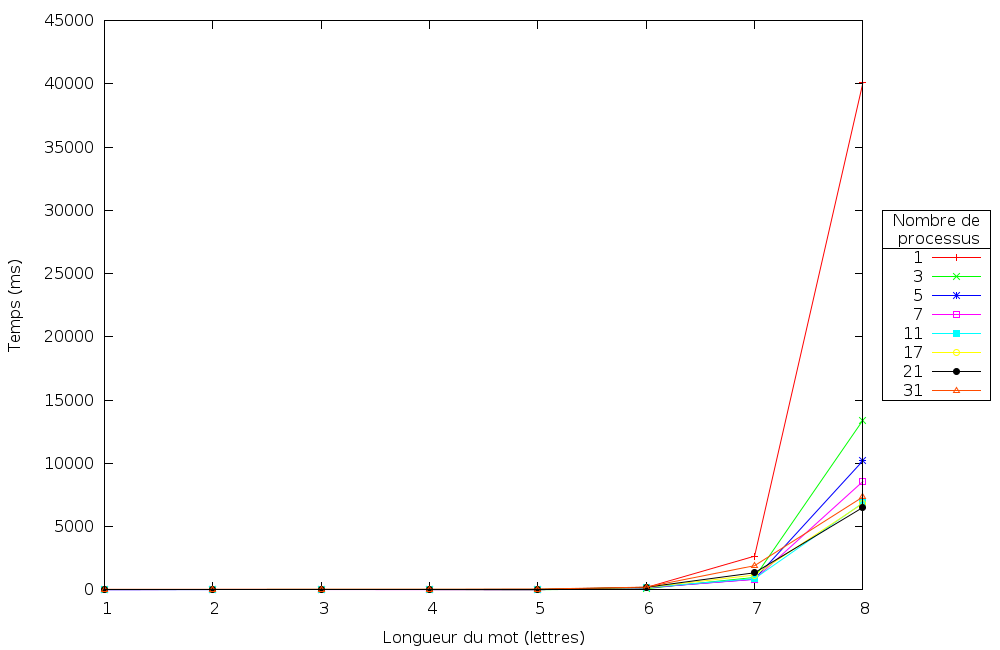
\includegraphics[width=\textwidth]{plot.png}
  \caption{Tests de performance}
  \label{perf}
\end{figure}

\section{Conclusion}




\end{document}
